\documentclass[main.tex]{subfiles}
\begin{document}
\section{Traditional Neutron Tagging}
Neutron tagging is done by time-correlating the detection of signals in the detectors. The NE213 detector is sensitive to both neutrons and gammas, whereas the YAPS are only sensitive to gammas. If a hit in the NE213 coincides (within some tolerance) with a hit in a YAP, then whave one count for our Time of flight spectrum. Some of these counts will be due to random coincidences, but the majority will be due to either $\gamma\gamma$ and n$\gamma$ pairs.

In the analog setup the NE213 acts as a start signal for the TDC, and the YAP signals are delayed so that they can act as stop signals.

\subsection{Schematic overview}
Signals in the NE213 detector are copied in a fan in fan out module. Two of these signals will be used to acquire longgate and shortgate integrals of the pulses. The third signal from the FIFO module is sent into a constant fraction discriminator, which starts a 50 ns square wave pulse when the cfd threshold is surpassed. 

%show scope trace of cfd.

This logic signal is then sent to a latch which switches state. For the next 10 $\mu$s, until the latch resets, no signals can pass through the latch. This way only one event is processed at a time. The downside to this is that a certain fraction of events are lost. scalers placed on either side of the latch make it possible to calculate this fraction for a given data set.

The signal is then copied again and reshaped. A 60 ns and a 500 ns square wave is used to define the qdc integration window for the copies of the analog NE213 signal mentioned above. A 150 ns square wave is used to define the integration window for the yap qdc, and another square wave triggers the start of a time of flight tdc.

The stop signal comes from the yap. The yap signals are sent into a linear fifo module, with one outgoing signal sent to a qdc, which triggers on the above mentioned NE213 signal. %yap qdc scope trace.
The other outgoing signal is sent to a cfd where a square pulse of 50 ns is produced. this pulse is then delayed by 300 ns and will act as the stop signal if a start signal is received from the NE213. %show tdc spectrum here?

\subsection{Analog data}
Over 4 hours of measurements $17.3\cdot 10^{6}$ events were recorded by the analog setup. The immediate output is 4 tdc spectrums Giving the time differences for NE213 hits and the respective YAPs. qdc spectra, one for each yap, and two qdc spectra for the NE213 detector (one longgate and one shortgate).

\newpage
\subsubsection{ToF spectrum}
\begin{figure}[ht]
    \centering
        \includegraphics[width=\textwidth]{AnalogResults/tof.pdf}
        \caption{The time of flight spectrum.}
    \label{fig:A_TOF}
\end{figure}

\newpage

\subsubsection{NE213 QDC spectrum}
The energy registered in the longgate QDC is shown in fig \ref{fig:qdc_a}. 'A peak is clearly visible at around 4.4 $MeV_{ec}$. This is the energy of the gammas emmited by the deexciting $^{12}C$ atoms. ---Write about other peak---
\begin{figure}[ht!]
    \centering
        \includegraphics[width=\textwidth]{AnalogResults/Ecall.png}
        \caption{Analog QDC spectrum calibration.}
    \label{fig:qdc_a}
\end{figure}

\newpage
\subsubsection{YAP QDC spectrum}
Write about scattered gammas that are both stop and start signals. Geometry dependent. Analog setup only records when there is a ToF coincidence, so scattered gammas end up dominating the yap qdc spectrum, which leads to the yap closest to the NE213 always having the largest gamma peak in the ToF spectrum. 

\newpage
\subsection{Pulse shape discrimination}
\subsubsection{Charge comparison method}
Since neutrons and gammas interact differently in the NE213 detector their signal has different shape and duration. This makes it possible to discriminate between neutrons and gammas.
\begin{figure}
    \centering
        \includegraphics[width=\textwidth]{AnalogResults/psd.pdf}
        \caption{Hexbin heatmap of Pulse shape distribution. The upper band is neutrons and the lower one is gammas.}
        \label{fig:hex_a}
\end{figure}

\subsection{Pulse shape v ToF}
\begin{figure}[ht]
    \centering
        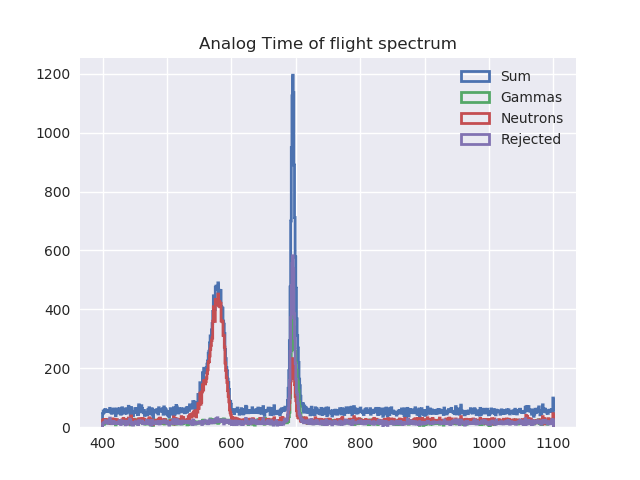
\includegraphics[width=\textwidth]{AnalogResults/tof_psd.pdf}
        \caption{heatmap of ToF vs pulse shape.}
    \label{fig:tof_ps_a} 
\end{figure}





\end{document}
